\documentclass[12pt,aspectratio=169]{beamer}
\usepackage{fancyvrb}
\RecustomVerbatimCommand{\VerbatimInput}{VerbatimInput}{frame=single,
numbersep=1mm, numbers=left, formatcom=\color{orange}}
%\usepackage{kpfonts}
%\usepackage[bitstream-charter]{mathdesign}
\usepackage[utf8]{inputenc}
\usepackage{pgf}
\usepackage{verbatim}
%\usepackage{fontspec}
\usepackage[ruled,vlined,linesnumbered]{algorithm2e}
\IncMargin{1em}
\usetheme{Madrid}
\setbeamerfont{frametitle}{series=\bfseries}
\usecolortheme[dark]{solarized}
\setbeamertemplate{blocks}[rounded][shadow=false]
\setbeamertemplate{navigation symbols}{}

\input{today.txt}

\author{Gianluca Della Vedova}
\title[Advanced Algorithms]{Advanced Techniques for Combinatorial Algorithms:
Approximation Algorithms}
\institute[]{Univ. Milano--Bicocca\\
  \texttt{https://gianluca.dellavedova.org}}
\date[]{{\tiny \today\hspace{1em} \vcsShortHash}}

\DeclareMathOperator{\poly}{\text{poly}}
\DeclareMathOperator{\polylog}{\text{polylog}}


% If you wish to uncover everything in a step-wise fashion, uncomment
% the following command:
% \beamerdefaultoverlayspecification{<+->}


\begin{document}

\begin{frame}
  \titlepage
\end{frame}


\begin{frame}\frametitle{Gianluca Della Vedova}
  \begin{itemize}
  \item
                Advanced Techniques for Combinatorial Algorithms
\item
{\small\url{https://gitlab.com/dellavg/advanced-algorithms}}
  \item
{\small\url{https://gianluca.dellavedova.org}}
  \item
{\small\url{gianluca.dellavedova@unimib.it}}
  \end{itemize}
\end{frame}

\begin{frame}\frametitle{NPO}
  \begin{block}{Optimization problem}
      \begin{itemize}
  \item
    Infinite set $\mathcal{I}$ of instances.
%
    The set $\mathcal{I}$ is recognizable in polynomial time
  \item
    For each instance $I\in\mathcal{I}$, the set $F(I)$ of feasible solutions.
%
    Each set $F(I)$ is recognizable in polynomial time.
%
    The set of all feasible solutions is $\mathcal{F}$
  \item
    An objective function $w: \mathcal{I} \times \mathcal{F}\mapsto \mathbb{Q}^{+}$.
%
    $w$ is a partial function --- $w(i,x)$ can be undefined if $x\notin F(i)$.
%
    $w$ is computable in polynomial time
  \item
    Goal: to minimize or to maximize
  \end{itemize}
\end{block}
\begin{block}{Approximation factor}
  $$\frac{APX}{OPT}$$
  APX: value of (approximate) feasible solution, OPT: value of best feasible solution
  \end{block}
\end{frame}

\begin{frame}\frametitle{Min Vertex Cover }
\begin{columns} 
  \begin{column}{0.48\textwidth}
  \begin{block}{Instance}
    Undirected graph $G=\langle V,E \rangle$
  \end{block}
  \begin{block}{Feasible solutions}
    A set $C\subset V$ such that for each edge $e\in E$ at least one endpoint of $e$
    belongs to $C$
  \end{block}
  \begin{block}{Objective function}
    $|C|$
  \end{block}
\end{column}
    
    \begin{column}{0.48\textwidth}
      \centering

  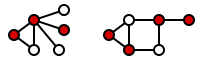
\includegraphics[height=0.2\textheight]{img/Vertex-cover}
\end{column}
\end{columns}
\end{frame}


\begin{frame}\frametitle{Max Clique }
\begin{columns} 
  \begin{column}{0.48\textwidth}
  \begin{block}{Instance}
    Undirected graph $G=\langle V,E \rangle$
  \end{block}
  \begin{block}{Feasible solution}
    Find a set $C\subset V$ such that all pairs of vertices in $C$ are connected by an edge
  \end{block}
    \begin{block}{Objective function}
      $|C|$
    \end{block}
  \end{column}
    
    \begin{column}{0.48\textwidth}
      \centering

  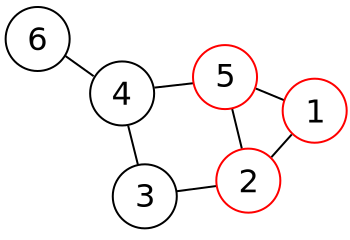
\includegraphics[height=0.5\textheight]{img/6n-graf-clique}
\end{column}
\end{columns}
\end{frame}

\begin{frame}\frametitle{Max Independent Set }
\begin{columns} 
  \begin{column}{0.48\textwidth}
  \begin{block}{Instance}
    Undirected graph $G=\langle V,E \rangle$
  \end{block}
  \begin{block}{Feasible solution}
    Find a set $I\subset V$ such that no two vertices in $K$ are connected by an edge
  \end{block}
    \begin{block}{Objective function}
      $|K|$
    \end{block}
  \end{column}
    
    \begin{column}{0.48\textwidth}
      \centering
  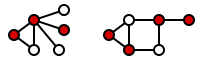
\includegraphics[height=0.2\textheight]{img/Vertex-cover}
\end{column}
\end{columns}
\end{frame}

\begin{frame}\frametitle{Max Cut }
\begin{columns} 
  \begin{column}{0.48\textwidth}
  \begin{block}{Instance}
    A weighted undirected  graph $G=\langle V,E \rangle$, $w:V\mapsto \mathbb{Q}^{+}$
  \end{block}
  \begin{block}{Feasible solution}
    a bipartition $(V_{1},V_{2})$ of $V$
  \end{block}
  \begin{block}{Objective function}
    $\sum_{v_{1}\in V_{1}, v_{2}\in V_{2}} w(v_{1}, v_{2})$
  \end{block}
\end{column}
    
    \begin{column}{0.48\textwidth}
      \centering
  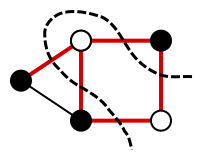
\includegraphics[height=0.7\textheight]{img/Max-cut}
\end{column}
\end{columns}
\end{frame}



\begin{frame}\frametitle{Min Traveling Salesperson (TSP)}
\begin{columns} 
  \begin{column}{0.48\textwidth}
  \begin{block}{Instance}
    A weighted undirected graph $G=\langle V,E \rangle$, $w:E\mapsto \mathbb{Q}^{+}$
  \end{block}
  \begin{block}{Feasible solution}
    Find a cycle $C$ that visits each vertex  $v\in V$ exactly once.
%
  \end{block}
  \begin{block}{Objective function}
    $\sum_{e\in C}w(e)$
  \end{block}
\end{column}
    \begin{column}{0.48\textwidth}
      \centering
  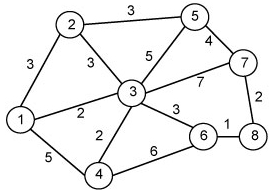
\includegraphics[height=0.5\textheight]{img/tsp}
\end{column}
\end{columns}
\end{frame}

\begin{frame}\frametitle{Min Set Cover }
\begin{columns} 
  \begin{column}{0.48\textwidth}
  \begin{block}{Instance}
    Universe set $U$, collection $\mathcal{S} = \{S_{1}, \ldots , S_{n}\}$of subsets of
    $U$.
    Weight $w: \mathcal{S}\mapsto \mathbb{Q}^{+}$
%
  \end{block}
  \begin{block}{Feasible solutions}
    A cover, that is a subcollection $\mathcal{C}$ of $\mathcal{S}$ that covers all elements of $U$
  \end{block}
  \begin{block}{Objective function}
    $\sum_{C\in \mathcal{C}} w(C)$
  \end{block}
\end{column}
    
    \begin{column}{0.48\textwidth}
      \centering

  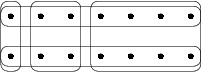
\includegraphics[height=0.2\textheight]{img/SetCoverGreedy}
\end{column}
\end{columns}
\end{frame}

\begin{frame}\frametitle{Min Set Cover }
\begin{columns} 
  \begin{column}{0.61\textwidth}
\begin{algorithm}[H]
  $C, D\gets \emptyset$\;
\While{$C\neq U$}
{
  $X\gets$ the set in $\mathcal{S}$ minimizing $w(X)/|X\setminus C|$\;
  $\alpha = \frac{w(X)}{|X\setminus C|}$\;
  Add $X$ to $D$\;
  For each $e\in C\setminus X$, $p(e)\gets \alpha$\;
  $C\gets C\cup X$
}
Output $D$
\caption{greedy-set-cover}
\end{algorithm}
\end{column}
  \begin{column}{0.34\textwidth}
\begin{block}{Lemma}
    $p(e_{k}) \le \frac{OPT}{n-k+1}$
  \end{block}
  \begin{block}{Corollary}
    Approximation factor is $1 + \frac{1}{2} + \frac{1}{2} + \cdots + \frac{1}{n} \le
    O(\log n)$
  \end{block}
\end{column}
\end{columns}
\end{frame}

\begin{frame}\frametitle{Min Metric Steiner Tree}
\begin{columns} 
  \begin{column}{0.48\textwidth}
  \begin{block}{Instance}
    A weighted undirected graph $G=\langle V,E \rangle$, $w:E\mapsto \mathbb{Q}^{+}$, $w$
    with triangle inequality.
%
    $V$ partition into $R$ (required) and $S$ (steiner)
  \end{block}
  \begin{block}{Feasible solution}
    A subtree $T$ of $G$ that includes all required vertices.
%
  \end{block}
  \begin{block}{Objective function}
    $\sum_{e\in T}w(e)$
  \end{block}
\end{column}
    \begin{column}{0.48\textwidth}
      \begin{block}{Approximation}
        Spanning tree $T$ of $G$
      \end{block}
      \begin{block}{2-approximation}
Euler tour of optimal solution $T^{*}$
      \end{block}
    \end{column}
\end{columns}
\end{frame}

\begin{frame}\frametitle{Min Metric Traveling Salesperson (TSP)}
\begin{columns} 
  \begin{column}{0.48\textwidth}
  \begin{block}{Instance}
    A weighted undirected graph $G=\langle V,E \rangle$, $w:E\mapsto \mathbb{Q}^{+}$, $w$
    with triangle inequality.
  \end{block}
  \begin{block}{Feasible solution}
    Find a cycle $C$ that visits each vertex  $v\in V$ exactly once.
%
  \end{block}
  \begin{block}{Objective function}
    $\sum_{e\in C}w(e)$
  \end{block}
\end{column}
    \begin{column}{0.48\textwidth}
      \begin{block}{2-approximation}
        Euler tour
      \end{block}
      \begin{block}{$\frac{3}{2}$-approximation}
Matching on odd-degree vertices of a spanning tree $T$
      \end{block}
    \end{column}
\end{columns}
\end{frame}

  \begin{frame}\frametitle{Shortest Superstring }
  \begin{block}{Instance}
      $s_{1}, \ldots, s_{m}$: strings of length $n$.
  \end{block}
  \begin{block}{Feasible solution}
    A superstring $T$, that is each $s_{i}$ is a substring of $T$
%
  \end{block}
  \begin{block}{Objective function}
    $|T|$
  \end{block}
\end{frame} 


  \begin{frame}\frametitle{Shortest Superstring }
  \begin{block}{Prefix graph}
      Arc $s_{i}, s_{j}$ with weight $pref(s_{i}, s_{j})$
  \end{block}
  \begin{block}{Length of superstring}
    Cycle of prefix graph + overlap last and first string
%
  \end{block}
  \begin{block}{Assignment problem = cycle cover}
    From $G=\langle V, E\rangle$ to $G_{2}$ with two copies $U$, $W$ of $V$.
%
    For each edge $(v_{i}, v_{j})\in E$, add two edges $(u_{i}, w_{i})$, $(w_{i}, u_{i})$
    to $G_{2}$
  \end{block}
  \begin{block}{Algorithm}
    \begin{itemize}
    \item
      Concatenate all cycle covers
    \item
      4-approximation
    \end{itemize}
  \end{block}
\end{frame} 


\begin{frame}\frametitle{Knapsack }
  \begin{block}{Instance}
    Universe set $U$, size $s: U \mapsto \mathbb{Z}^{+}$, profit $p: U \mapsto
    \mathbb{Z}^{+}$, capacity $B\in \mathbb{Z}^{+}$
%
  \end{block}
  \begin{block}{Feasible solutions}
    A subset $K\subseteq U$, such that $\sum_{k\in K}s(k) \le B$
  \end{block}
  \begin{block}{Objective function}
    $\sum_{k\in K} p(k)$, to maximize
  \end{block}
\end{frame}


\begin{frame}\frametitle{Knapsack }
  \begin{block}{Algorithm}
    \begin{itemize}[<.->]
    \item
      Dynamic programming
    \item
      NP-hard
    \item
      $K(i,b)$: uses only $\{u_{1}, \ldots, u_{i}\}$, total size $b$
    \item
      pseudo-polynomial time
    \item
      Transform it into an approximation algorithm
    \item
      Scale down profits $p_{1}(u) = \lfloor p(u) \frac{n}{\epsilon \max\{p(u)\}} \rfloor$, move to dual problem
    \item
      Approximation factor $1-\epsilon$, $\forall \epsilon>0$
    \item
      Time polynomial in $n$ and $\frac{1}{\epsilon}$
    \item
      \emph{FPTAS}
    \end{itemize}
  \end{block}
\end{frame} 

% \begin{frame}\frametitle{Bin Packing }
%   \begin{block}{Instance}
%     Universe set $U$, size $s: U \mapsto \mathbb{Q}^{+}$, $s(u)< 1 \forall u\in U$
% %
%   \end{block}
%   \begin{block}{Feasible solutions}
%     A partition $P$ of $U$ such that the sum $\sum_{u\in C} s(u) \le 1$ for each class
%   $C$ of the partition $P$
%   \end{block}
%   \begin{block}{Objective function}
%     the number of classes of $P$, to minimize
%   \end{block}
% \end{frame} 


\begin{frame}\frametitle{Attribution}
\small
  \begin{itemize}[<.->]
  \item
    Vertex Cover figure: By Miym - Own work, CC BY-SA 3.0,
    \url{https://commons.wikimedia.org/w/index.php?curid=6017739}
  \item
    Clique figure: Public Domain,
    \url{https://commons.wikimedia.org/w/index.php?curid=1072101}
  \item
    Max Cut figure: By Miym - Own work, CC BY-SA 3.0,
    \url{https://commons.wikimedia.org/w/index.php?curid=6002348}
  \item
    Set Cover figure: Public Domain, \url{https://commons.wikimedia.org/w/index.php?curid=647030}
  \end{itemize}
\end{frame}

\end{document}
%%% Local Variables:
%%% mode: latex
%%% TeX-PDF-mode: t
%%% buffer-file-coding-system: utf-8
%%% End:
